%\documentclass[a4paper,11pt,twoside]{article}
%\usepackage{graphicx}
%\begin{document}

\begin{figure}[h]
	\centering
	
\includegraphics[width=0.5\linewidth]{Grafik/Diagramm/Pattern/ClientServer/Kontext.png}
	\caption[]{Client-Server-Modell}
\end{figure}

\subsection*{Client}
Der Client ist der User, der Datensätze, Algorithmen auf den Server hochladen, diese dann dort berechnen lassen und Pakete downloaden kann.

\subsection*{Server}
Der Server bietet dem User den Dienst an, Modelle anhand von schon vorhandenen oder vom User hoch geladenen Datensätzen und Algorithmen zu erstellen. Des Weiteren dient der Server als Datenbank von schon mit verschiedenen Datensätzen erstellten Modellen.\\

\begin{figure}[h]
	\centering
	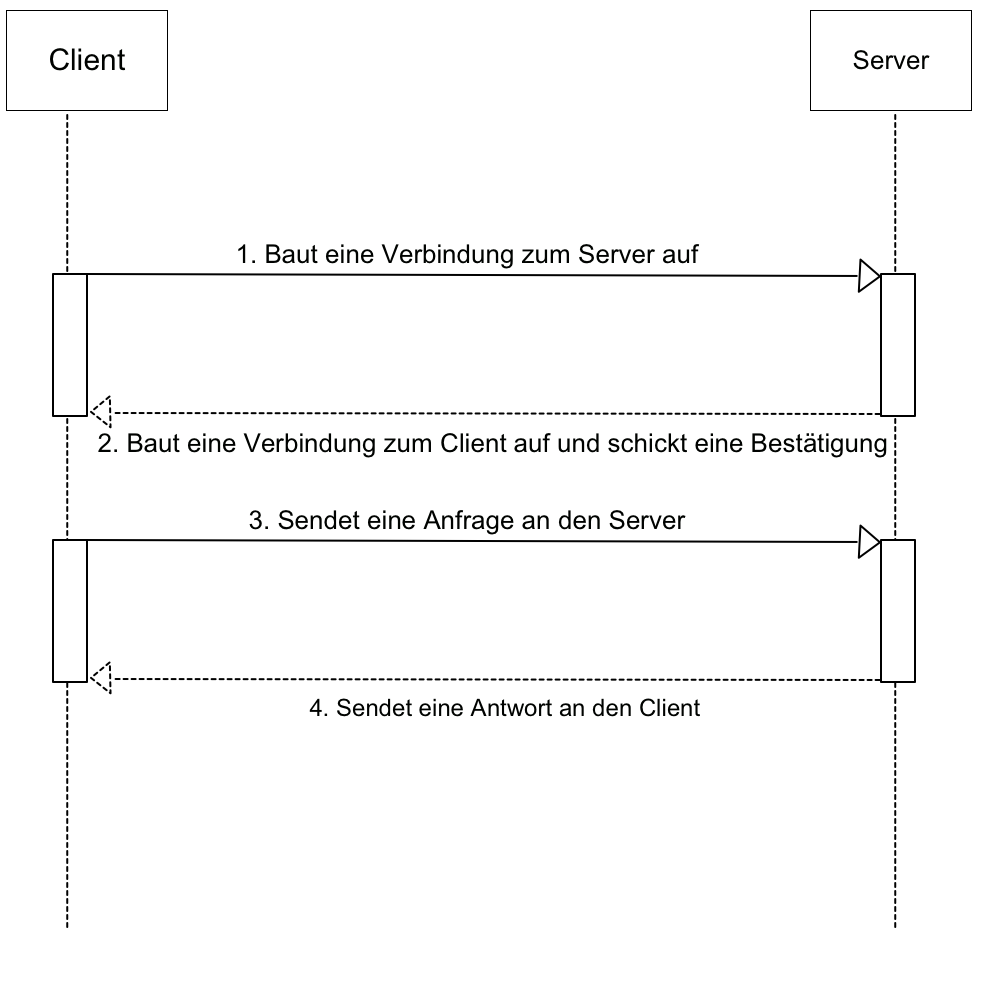
\includegraphics[width=0.6\linewidth]{Grafik/Diagramm/Pattern/ClientServer/Sequenzdiagramm.png}
	\caption[]{Client-Server-Sequenzdiagramm}
\end{figure}\pagebreak
Der Client versucht eine Verbindung zum Server aufzubauen, der Server versucht ebenfalls bei Anfrage eine Verbindung zum Client Aufzubauen und schickt dem Client eine Bestätigung, das die Verbindung steht. Danach kann der Client Datensätze/Algorithmen hochladen und dem Server eine Anfrage zum Modelle downloaden schicken.

\subsection*{Was spricht für das Client-Server-Modell?}
Das Client-Server-Modell wird verwendet, wenn eine Datenbank oder ein Service von verschiedenen Orten her abgerufen werden soll. Dies ist für beides der Fall. Der User kann global auf den Server zugreifen und Daten hoch und runter laden.\\
Des Weiteren sollen mehrere gleiche Server online sein, damit viele User-anfragen auf mehrere Server verteilt werden können und somit schneller bearbeitet werden können. Der User sieht aber nur den einen Server. Wenn ein Server offline (ausfällt/gewartet)ist und es sind mehrere online, so bekommt der User davon nichts mit und wird auf einen anderen Server geleitet.\\
Nachteile sind:\\
-Die Leistung des Systems ist unberechenbar, wenn die verschiedenen Service im Server-Netzwerk verteilt ist. Dieser Fall existiert in unserem System nicht.\\
-Es gibt Management Probleme, wenn Server in relativ Unabhängigen Besitz ist. Da die Server unabhängig arbeiten und nur zusammenarbeiten, wenn schon vorhandene Modelle/Datensätze auf einem anderen Server angefragt werden, ist dieser Nachteil zu vernachlässigen.





%\end{document}